\documentclass[1p]{elsarticle_modified}
%\bibliographystyle{elsarticle-num}

%\usepackage[colorlinks]{hyperref}
%\usepackage{abbrmath_seonhwa} %\Abb, \Ascr, \Acal ,\Abf, \Afrak
\usepackage{amsfonts}
\usepackage{amssymb}
\usepackage{amsmath}
\usepackage{amsthm}
\usepackage{scalefnt}
\usepackage{amsbsy}
\usepackage{kotex}
\usepackage{caption}
\usepackage{subfig}
\usepackage{color}
\usepackage{graphicx}
\usepackage{xcolor} %% white, black, red, green, blue, cyan, magenta, yellow
\usepackage{float}
\usepackage{setspace}
\usepackage{hyperref}

\usepackage{tikz}
\usetikzlibrary{arrows}

\usepackage{multirow}
\usepackage{array} % fixed length table
\usepackage{hhline}

%%%%%%%%%%%%%%%%%%%%%
\makeatletter
\renewcommand*\env@matrix[1][\arraystretch]{%
	\edef\arraystretch{#1}%
	\hskip -\arraycolsep
	\let\@ifnextchar\new@ifnextchar
	\array{*\c@MaxMatrixCols c}}
\makeatother %https://tex.stackexchange.com/questions/14071/how-can-i-increase-the-line-spacing-in-a-matrix
%%%%%%%%%%%%%%%

\usepackage[normalem]{ulem}

\newcommand{\msout}[1]{\ifmmode\text{\sout{\ensuremath{#1}}}\else\sout{#1}\fi}
%SOURCE: \msout is \stkout macro in https://tex.stackexchange.com/questions/20609/strikeout-in-math-mode

\newcommand{\cancel}[1]{
	\ifmmode
	{\color{red}\msout{#1}}
	\else
	{\color{red}\sout{#1}}
	\fi
}

\newcommand{\add}[1]{
	{\color{blue}\uwave{#1}}
}

\newcommand{\replace}[2]{
	\ifmmode
	{\color{red}\msout{#1}}{\color{blue}\uwave{#2}}
	\else
	{\color{red}\sout{#1}}{\color{blue}\uwave{#2}}
	\fi
}

\newcommand{\Sol}{\mathcal{S}} %segment
\newcommand{\D}{D} %diagram
\newcommand{\A}{\mathcal{A}} %arc


%%%%%%%%%%%%%%%%%%%%%%%%%%%%%5 test

\def\sl{\operatorname{\textup{SL}}(2,\Cbb)}
\def\psl{\operatorname{\textup{PSL}}(2,\Cbb)}
\def\quan{\mkern 1mu \triangleright \mkern 1mu}

\theoremstyle{definition}
\newtheorem{thm}{Theorem}[section]
\newtheorem{prop}[thm]{Proposition}
\newtheorem{lem}[thm]{Lemma}
\newtheorem{ques}[thm]{Question}
\newtheorem{cor}[thm]{Corollary}
\newtheorem{defn}[thm]{Definition}
\newtheorem{exam}[thm]{Example}
\newtheorem{rmk}[thm]{Remark}
\newtheorem{alg}[thm]{Algorithm}

\newcommand{\I}{\sqrt{-1}}
\begin{document}

%\begin{frontmatter}
%
%\title{Boundary parabolic representations of knots up to 8 crossings}
%
%%% Group authors per affiliation:
%\author{Yunhi Cho} 
%\address{Department of Mathematics, University of Seoul, Seoul, Korea}
%\ead{yhcho@uos.ac.kr}
%
%
%\author{Seonhwa Kim} %\fnref{s_kim}}
%\address{Center for Geometry and Physics, Institute for Basic Science, Pohang, 37673, Korea}
%\ead{ryeona17@ibs.re.kr}
%
%\author{Hyuk Kim}
%\address{Department of Mathematical Sciences, Seoul National University, Seoul 08826, Korea}
%\ead{hyukkim@snu.ac.kr}
%
%\author{Seokbeom Yoon}
%\address{Department of Mathematical Sciences, Seoul National University, Seoul, 08826,  Korea}
%\ead{sbyoon15@snu.ac.kr}
%
%\begin{abstract}
%We find all boundary parabolic representation of knots up to 8 crossings.
%
%\end{abstract}
%\begin{keyword}
%    \MSC[2010] 57M25 
%\end{keyword}
%
%\end{frontmatter}

%\linenumbers
%\tableofcontents
%
\newcommand\colored[1]{\textcolor{white}{\rule[-0.35ex]{0.8em}{1.4ex}}\kern-0.8em\color{red} #1}%
%\newcommand\colored[1]{\textcolor{white}{ #1}\kern-2.17ex	\textcolor{white}{ #1}\kern-1.81ex	\textcolor{white}{ #1}\kern-2.15ex\color{red}#1	}

{\Large $\underline{12a_{0830}~(K12a_{0830})}$}

\setlength{\tabcolsep}{10pt}
\renewcommand{\arraystretch}{1.6}
\vspace{1cm}\begin{tabular}{m{100pt}>{\centering\arraybackslash}m{274pt}}
\multirow{5}{120pt}{
	\centering
	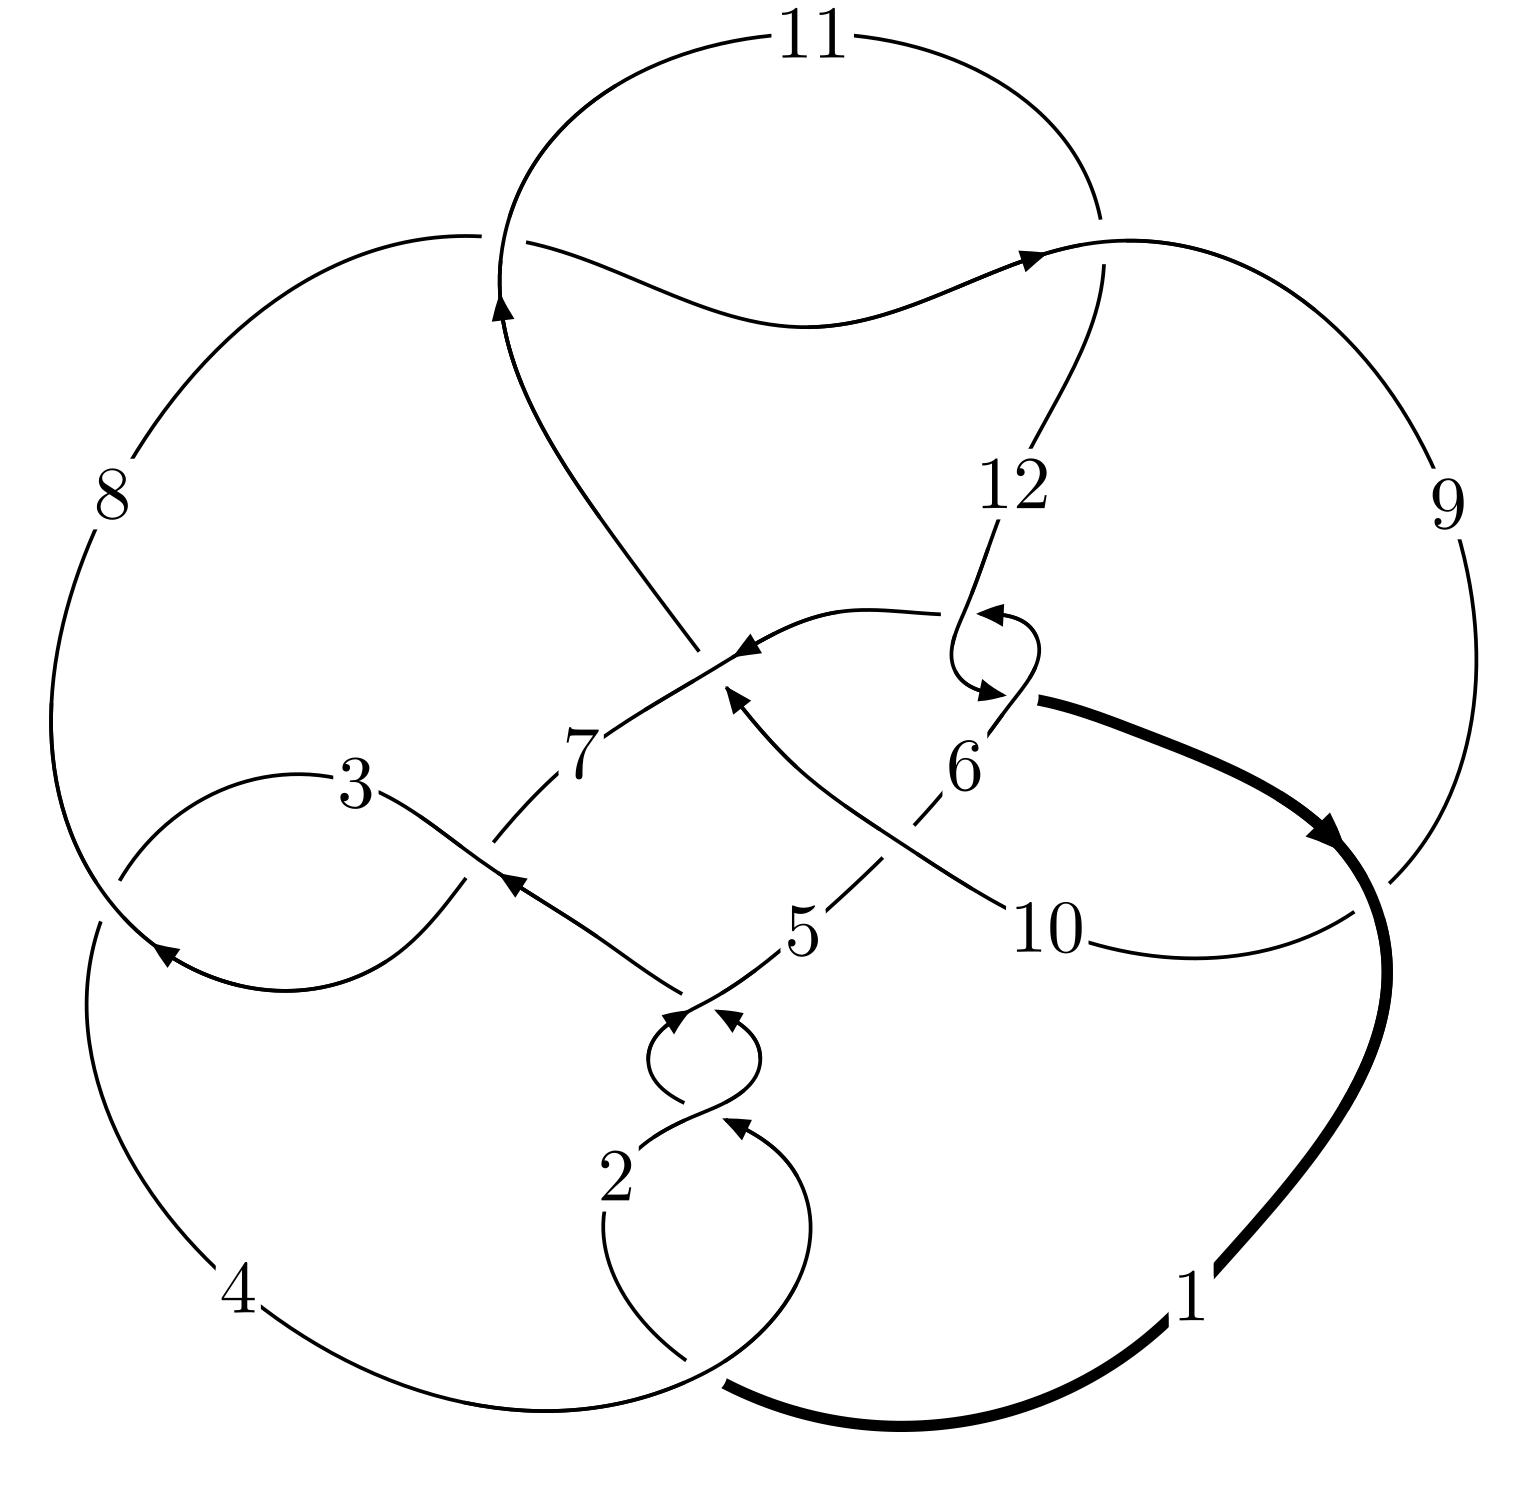
\includegraphics[width=112pt]{../../../GIT/diagram.site/Diagrams/png/1631_12a_0830.png}\\
\ \ \ A knot diagram\footnotemark}&
\allowdisplaybreaks
\textbf{Linearized knot diagam} \\
\cline{2-2}
 &
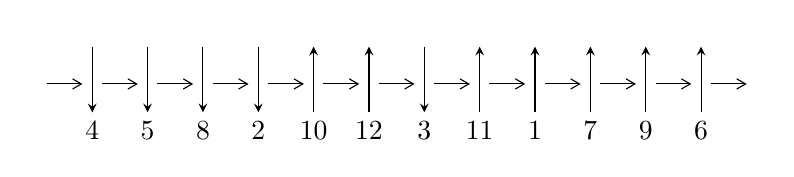
\begin{tikzpicture}[x=20pt, y=17pt]
	% nodes
	\node (C0) at (0, 0) {};
	\node (C1) at (1, 0) {};
	\node (C1U) at (1, +1) {};
	\node (C1D) at (1, -1) {4};

	\node (C2) at (2, 0) {};
	\node (C2U) at (2, +1) {};
	\node (C2D) at (2, -1) {5};

	\node (C3) at (3, 0) {};
	\node (C3U) at (3, +1) {};
	\node (C3D) at (3, -1) {8};

	\node (C4) at (4, 0) {};
	\node (C4U) at (4, +1) {};
	\node (C4D) at (4, -1) {2};

	\node (C5) at (5, 0) {};
	\node (C5U) at (5, +1) {};
	\node (C5D) at (5, -1) {10};

	\node (C6) at (6, 0) {};
	\node (C6U) at (6, +1) {};
	\node (C6D) at (6, -1) {12};

	\node (C7) at (7, 0) {};
	\node (C7U) at (7, +1) {};
	\node (C7D) at (7, -1) {3};

	\node (C8) at (8, 0) {};
	\node (C8U) at (8, +1) {};
	\node (C8D) at (8, -1) {11};

	\node (C9) at (9, 0) {};
	\node (C9U) at (9, +1) {};
	\node (C9D) at (9, -1) {1};

	\node (C10) at (10, 0) {};
	\node (C10U) at (10, +1) {};
	\node (C10D) at (10, -1) {7};

	\node (C11) at (11, 0) {};
	\node (C11U) at (11, +1) {};
	\node (C11D) at (11, -1) {9};

	\node (C12) at (12, 0) {};
	\node (C12U) at (12, +1) {};
	\node (C12D) at (12, -1) {6};
	\node (C13) at (13, 0) {};

	% arrows
	\draw[->,>={angle 60}]
	(C0) edge (C1) (C1) edge (C2) (C2) edge (C3) (C3) edge (C4) (C4) edge (C5) (C5) edge (C6) (C6) edge (C7) (C7) edge (C8) (C8) edge (C9) (C9) edge (C10) (C10) edge (C11) (C11) edge (C12) (C12) edge (C13) ;	\draw[->,>=stealth]
	(C1U) edge (C1D) (C2U) edge (C2D) (C3U) edge (C3D) (C4U) edge (C4D) (C5D) edge (C5U) (C6D) edge (C6U) (C7U) edge (C7D) (C8D) edge (C8U) (C9D) edge (C9U) (C10D) edge (C10U) (C11D) edge (C11U) (C12D) edge (C12U) ;
	\end{tikzpicture} \\
\hhline{~~} \\& 
\textbf{Solving Sequence} \\ \cline{2-2} 
 &
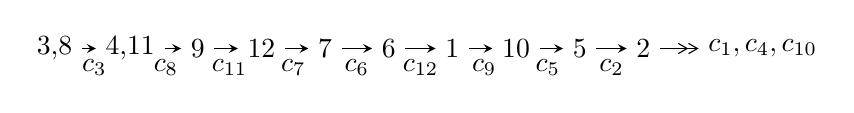
\begin{tikzpicture}[x=23pt, y=7pt]
	% node
	\node (A0) at (-1/8, 0) {3,8};
	\node (A1) at (17/16, 0) {4,11};
	\node (A2) at (17/8, 0) {9};
	\node (A3) at (25/8, 0) {12};
	\node (A4) at (33/8, 0) {7};
	\node (A5) at (41/8, 0) {6};
	\node (A6) at (49/8, 0) {1};
	\node (A7) at (57/8, 0) {10};
	\node (A8) at (65/8, 0) {5};
	\node (A9) at (73/8, 0) {2};
	\node (C1) at (1/2, -1) {$c_{3}$};
	\node (C2) at (13/8, -1) {$c_{8}$};
	\node (C3) at (21/8, -1) {$c_{11}$};
	\node (C4) at (29/8, -1) {$c_{7}$};
	\node (C5) at (37/8, -1) {$c_{6}$};
	\node (C6) at (45/8, -1) {$c_{12}$};
	\node (C7) at (53/8, -1) {$c_{9}$};
	\node (C8) at (61/8, -1) {$c_{5}$};
	\node (C9) at (69/8, -1) {$c_{2}$};
	\node (A10) at (11, 0) {$c_{1},c_{4},c_{10}$};

	% edge
	\draw[->,>=stealth]	
	(A0) edge (A1) (A1) edge (A2) (A2) edge (A3) (A3) edge (A4) (A4) edge (A5) (A5) edge (A6) (A6) edge (A7) (A7) edge (A8) (A8) edge (A9) ;
	\draw[->>,>={angle 60}]	
	(A9) edge (A10);
\end{tikzpicture} \\ 

\end{tabular} \\

\footnotetext{
The image of knot diagram is generated by the software ``\textbf{Draw programme}" developed by Andrew Bartholomew(\url{http://www.layer8.co.uk/maths/draw/index.htm\#Running-draw}), where we modified some parts for our purpose(\url{https://github.com/CATsTAILs/LinksPainter}).
}\phantom \\ \newline 
\centering \textbf{Ideals for irreducible components\footnotemark of $X_{\text{par}}$} 
 
\begin{align*}
I^u_{1}&=\langle 
-1.45248\times10^{403} u^{112}+2.57534\times10^{403} u^{111}+\cdots+7.60655\times10^{404} b-1.41148\times10^{405},\\
\phantom{I^u_{1}}&\phantom{= \langle  }-3.58295\times10^{402} u^{112}+6.66928\times10^{402} u^{111}+\cdots+8.94888\times10^{403} a-1.02347\times10^{405},\\
\phantom{I^u_{1}}&\phantom{= \langle  }u^{113}-2 u^{112}+\cdots+896 u-256\rangle \\
I^u_{2}&=\langle 
-22 u^2+17 b+15 u-40,\;- u^2+a+u-2,\;u^3- u^2+2 u-1\rangle \\
\\
I^v_{1}&=\langle 
a,\;72 v^7-466 v^6-1954 v^5+4124 v^4+13122 v^3-3530 v^2+887 b-5049 v+2666,\\
\phantom{I^v_{1}}&\phantom{= \langle  }v^8+3 v^7-7 v^6-28 v^5-13 v^4+8 v^3-2 v+1\rangle \\
\end{align*}
\raggedright * 3 irreducible components of $\dim_{\mathbb{C}}=0$, with total 124 representations.\\
\footnotetext{All coefficients of polynomials are rational numbers. But the coefficients are sometimes approximated in decimal forms when there is not enough margin.}
\newpage
\renewcommand{\arraystretch}{1}
\centering \section*{I. $I^u_{1}= \langle -1.45\times10^{403} u^{112}+2.58\times10^{403} u^{111}+\cdots+7.61\times10^{404} b-1.41\times10^{405},\;-3.58\times10^{402} u^{112}+6.67\times10^{402} u^{111}+\cdots+8.95\times10^{403} a-1.02\times10^{405},\;u^{113}-2 u^{112}+\cdots+896 u-256 \rangle$}
\flushleft \textbf{(i) Arc colorings}\\
\begin{tabular}{m{7pt} m{180pt} m{7pt} m{180pt} }
\flushright $a_{3}=$&$\begin{pmatrix}1\\0\end{pmatrix}$ \\
\flushright $a_{8}=$&$\begin{pmatrix}0\\u\end{pmatrix}$ \\
\flushright $a_{4}=$&$\begin{pmatrix}1\\u^2\end{pmatrix}$ \\
\flushright $a_{11}=$&$\begin{pmatrix}0.0400380 u^{112}-0.0745263 u^{111}+\cdots+1.44165 u+11.4369\\0.0190951 u^{112}-0.0338568 u^{111}+\cdots+5.71448 u+1.85561\end{pmatrix}$ \\
\flushright $a_{9}=$&$\begin{pmatrix}-0.00768519 u^{112}+0.0258094 u^{111}+\cdots-28.2706 u+7.32413\\0.0215710 u^{112}-0.0343632 u^{111}+\cdots-2.70707 u+4.95920\end{pmatrix}$ \\
\flushright $a_{12}=$&$\begin{pmatrix}0.0166558 u^{112}-0.0116771 u^{111}+\cdots-31.1306 u+11.0180\\-0.00139532 u^{112}+0.00197886 u^{111}+\cdots+4.41793 u-1.91206\end{pmatrix}$ \\
\flushright $a_{7}=$&$\begin{pmatrix}u\\u\end{pmatrix}$ \\
\flushright $a_{6}=$&$\begin{pmatrix}-0.0623893 u^{112}+0.0719018 u^{111}+\cdots+82.4207 u-33.2834\\-0.0116805 u^{112}+0.0134724 u^{111}+\cdots+15.8056 u-5.85623\end{pmatrix}$ \\
\flushright $a_{1}=$&$\begin{pmatrix}0.0408769 u^{112}-0.0373320 u^{111}+\cdots-84.9975 u+34.3053\\0.0107707 u^{112}-0.0171522 u^{111}+\cdots-3.86228 u+2.98419\end{pmatrix}$ \\
\flushright $a_{10}=$&$\begin{pmatrix}0.0397259 u^{112}-0.0772883 u^{111}+\cdots+5.71328 u+11.7482\\0.0187830 u^{112}-0.0366188 u^{111}+\cdots+9.98611 u+2.16697\end{pmatrix}$ \\
\flushright $a_{5}=$&$\begin{pmatrix}-0.0428338 u^{112}+0.0321310 u^{111}+\cdots+110.473 u-42.6931\\-0.00195693 u^{112}-0.00520094 u^{111}+\cdots+25.4752 u-8.38781\end{pmatrix}$ \\
\flushright $a_{2}=$&$\begin{pmatrix}0.0428338 u^{112}-0.0321310 u^{111}+\cdots-110.473 u+42.6931\\0.00867147 u^{112}-0.0107891 u^{111}+\cdots-11.5282 u+5.31757\end{pmatrix}$\\&\end{tabular}
\flushleft \textbf{(ii) Obstruction class $= -1$}\\~\\
\flushleft \textbf{(iii) Cusp Shapes $= 0.146247 u^{112}-0.233542 u^{111}+\cdots-65.9092 u+69.0820$}\\~\\
\newpage\renewcommand{\arraystretch}{1}
\flushleft \textbf{(iv) u-Polynomials at the component}\newline \\
\begin{tabular}{m{50pt}|m{274pt}}
Crossings & \hspace{64pt}u-Polynomials at each crossing \\
\hline $$\begin{aligned}c_{1},c_{2},c_{4}\end{aligned}$$&$\begin{aligned}
&u^{113}-10 u^{112}+\cdots+u-1
\end{aligned}$\\
\hline $$\begin{aligned}c_{3},c_{7}\end{aligned}$$&$\begin{aligned}
&u^{113}-2 u^{112}+\cdots+896 u-256
\end{aligned}$\\
\hline $$\begin{aligned}c_{5}\end{aligned}$$&$\begin{aligned}
&u^{113}+2 u^{112}+\cdots-41820 u-2312
\end{aligned}$\\
\hline $$\begin{aligned}c_{6},c_{12}\end{aligned}$$&$\begin{aligned}
&u^{113}+3 u^{112}+\cdots+3 u+1
\end{aligned}$\\
\hline $$\begin{aligned}c_{8},c_{11}\end{aligned}$$&$\begin{aligned}
&u^{113}+5 u^{112}+\cdots-1158 u+289
\end{aligned}$\\
\hline $$\begin{aligned}c_{9}\end{aligned}$$&$\begin{aligned}
&17(17 u^{113}+219 u^{112}+\cdots+16199 u+2539)
\end{aligned}$\\
\hline $$\begin{aligned}c_{10}\end{aligned}$$&$\begin{aligned}
&17(17 u^{113}+212 u^{112}+\cdots-115224 u-34421)
\end{aligned}$\\
\hline
\end{tabular}\\~\\
\newpage\renewcommand{\arraystretch}{1}
\flushleft \textbf{(v) Riley Polynomials at the component}\newline \\
\begin{tabular}{m{50pt}|m{274pt}}
Crossings & \hspace{64pt}Riley Polynomials at each crossing \\
\hline $$\begin{aligned}c_{1},c_{2},c_{4}\end{aligned}$$&$\begin{aligned}
&y^{113}-100 y^{112}+\cdots-13 y-1
\end{aligned}$\\
\hline $$\begin{aligned}c_{3},c_{7}\end{aligned}$$&$\begin{aligned}
&y^{113}-48 y^{112}+\cdots+1425408 y-65536
\end{aligned}$\\
\hline $$\begin{aligned}c_{5}\end{aligned}$$&$\begin{aligned}
&y^{113}+18 y^{112}+\cdots+117380240 y-5345344
\end{aligned}$\\
\hline $$\begin{aligned}c_{6},c_{12}\end{aligned}$$&$\begin{aligned}
&y^{113}+61 y^{112}+\cdots+19 y-1
\end{aligned}$\\
\hline $$\begin{aligned}c_{8},c_{11}\end{aligned}$$&$\begin{aligned}
&y^{113}-69 y^{112}+\cdots+10227136 y-83521
\end{aligned}$\\
\hline $$\begin{aligned}c_{9}\end{aligned}$$&$\begin{aligned}
&289(289 y^{113}+6473 y^{112}+\cdots-3.80828\times10^{8} y-6446521)
\end{aligned}$\\
\hline $$\begin{aligned}c_{10}\end{aligned}$$&$\begin{aligned}
&289(289 y^{113}-1016 y^{112}+\cdots-6.58097\times10^{9} y-1.18481\times10^{9})
\end{aligned}$\\
\hline
\end{tabular}\\~\\
\newpage\flushleft \textbf{(vi) Complex Volumes and Cusp Shapes}
$$\begin{array}{c|c|c}  
\text{Solutions to }I^u_{1}& \I (\text{vol} + \sqrt{-1}CS) & \text{Cusp shape}\\
 \hline 
\begin{aligned}
u &= -0.838996 + 0.519691 I \\
a &= -1.00735 - 0.99352 I \\
b &= -0.72221 - 1.67273 I\end{aligned}
 & \phantom{-}2.81518 + 2.25501 I & \phantom{-0.000000 } 0 \\ \hline\begin{aligned}
u &= -0.838996 - 0.519691 I \\
a &= -1.00735 + 0.99352 I \\
b &= -0.72221 + 1.67273 I\end{aligned}
 & \phantom{-}2.81518 - 2.25501 I & \phantom{-0.000000 } 0 \\ \hline\begin{aligned}
u &= -0.408038 + 0.896770 I \\
a &= \phantom{-}1.006650 + 0.985618 I \\
b &= -0.287546 + 0.217220 I\end{aligned}
 & \phantom{-}2.05403 - 8.53878 I & \phantom{-0.000000 } 0 \\ \hline\begin{aligned}
u &= -0.408038 - 0.896770 I \\
a &= \phantom{-}1.006650 - 0.985618 I \\
b &= -0.287546 - 0.217220 I\end{aligned}
 & \phantom{-}2.05403 + 8.53878 I & \phantom{-0.000000 } 0 \\ \hline\begin{aligned}
u &= \phantom{-}0.991916 + 0.215082 I \\
a &= -0.462328 - 0.945148 I \\
b &= -0.14976 - 2.01843 I\end{aligned}
 & -5.58135 - 3.04071 I & \phantom{-0.000000 } 0 \\ \hline\begin{aligned}
u &= \phantom{-}0.991916 - 0.215082 I \\
a &= -0.462328 + 0.945148 I \\
b &= -0.14976 + 2.01843 I\end{aligned}
 & -5.58135 + 3.04071 I & \phantom{-0.000000 } 0 \\ \hline\begin{aligned}
u &= \phantom{-}0.866741 + 0.411780 I \\
a &= -0.140138 + 0.673956 I \\
b &= \phantom{-}0.45614 + 1.69373 I\end{aligned}
 & -4.97488 + 1.61721 I & \phantom{-0.000000 } 0 \\ \hline\begin{aligned}
u &= \phantom{-}0.866741 - 0.411780 I \\
a &= -0.140138 - 0.673956 I \\
b &= \phantom{-}0.45614 - 1.69373 I\end{aligned}
 & -4.97488 - 1.61721 I & \phantom{-0.000000 } 0 \\ \hline\begin{aligned}
u &= \phantom{-}0.882043 + 0.367780 I \\
a &= \phantom{-}0.916925 - 0.363319 I \\
b &= \phantom{-}5.05394 - 4.27372 I\end{aligned}
 & -0.45862 - 1.47435 I & \phantom{-0.000000 } 0 \\ \hline\begin{aligned}
u &= \phantom{-}0.882043 - 0.367780 I \\
a &= \phantom{-}0.916925 + 0.363319 I \\
b &= \phantom{-}5.05394 + 4.27372 I\end{aligned}
 & -0.45862 + 1.47435 I & \phantom{-0.000000 } 0\\
 \hline 
 \end{array}$$\newpage$$\begin{array}{c|c|c}  
\text{Solutions to }I^u_{1}& \I (\text{vol} + \sqrt{-1}CS) & \text{Cusp shape}\\
 \hline 
\begin{aligned}
u &= -0.950581 + 0.000527 I \\
a &= \phantom{-}0.174135 - 0.403894 I \\
b &= -0.251243 - 0.903353 I\end{aligned}
 & -1.61934 - 0.33597 I & \phantom{-0.000000 } 0 \\ \hline\begin{aligned}
u &= -0.950581 - 0.000527 I \\
a &= \phantom{-}0.174135 + 0.403894 I \\
b &= -0.251243 + 0.903353 I\end{aligned}
 & -1.61934 + 0.33597 I & \phantom{-0.000000 } 0 \\ \hline\begin{aligned}
u &= -0.264647 + 1.026570 I \\
a &= -0.547724 + 0.190022 I \\
b &= \phantom{-}0.072210 + 0.674929 I\end{aligned}
 & -3.04736 - 1.94290 I & \phantom{-0.000000 } 0 \\ \hline\begin{aligned}
u &= -0.264647 - 1.026570 I \\
a &= -0.547724 - 0.190022 I \\
b &= \phantom{-}0.072210 - 0.674929 I\end{aligned}
 & -3.04736 + 1.94290 I & \phantom{-0.000000 } 0 \\ \hline\begin{aligned}
u &= -0.770530 + 0.533723 I \\
a &= -1.34205 - 0.86042 I \\
b &= -0.491734 - 0.873041 I\end{aligned}
 & \phantom{-}3.01974 + 2.02401 I & \phantom{-0.000000 } 0 \\ \hline\begin{aligned}
u &= -0.770530 - 0.533723 I \\
a &= -1.34205 + 0.86042 I \\
b &= -0.491734 + 0.873041 I\end{aligned}
 & \phantom{-}3.01974 - 2.02401 I & \phantom{-0.000000 } 0 \\ \hline\begin{aligned}
u &= \phantom{-}0.916425 + 0.542126 I \\
a &= \phantom{-}0.543187 - 1.265160 I \\
b &= \phantom{-}1.04849 - 2.00825 I\end{aligned}
 & \phantom{-}1.51696 - 5.57365 I & \phantom{-0.000000 } 0 \\ \hline\begin{aligned}
u &= \phantom{-}0.916425 - 0.542126 I \\
a &= \phantom{-}0.543187 + 1.265160 I \\
b &= \phantom{-}1.04849 + 2.00825 I\end{aligned}
 & \phantom{-}1.51696 + 5.57365 I & \phantom{-0.000000 } 0 \\ \hline\begin{aligned}
u &= -0.412108 + 0.839424 I \\
a &= -1.25948 - 0.65985 I \\
b &= -0.650987 + 0.011237 I\end{aligned}
 & -1.33451 - 3.90121 I & \phantom{-0.000000 } 0 \\ \hline\begin{aligned}
u &= -0.412108 - 0.839424 I \\
a &= -1.25948 + 0.65985 I \\
b &= -0.650987 - 0.011237 I\end{aligned}
 & -1.33451 + 3.90121 I & \phantom{-0.000000 } 0\\
 \hline 
 \end{array}$$\newpage$$\begin{array}{c|c|c}  
\text{Solutions to }I^u_{1}& \I (\text{vol} + \sqrt{-1}CS) & \text{Cusp shape}\\
 \hline 
\begin{aligned}
u &= \phantom{-}0.421431 + 0.994250 I \\
a &= -0.613154 + 0.932683 I \\
b &= \phantom{-}0.151544 + 0.326452 I\end{aligned}
 & \phantom{-}5.67260 + 2.25032 I & \phantom{-0.000000 } 0 \\ \hline\begin{aligned}
u &= \phantom{-}0.421431 - 0.994250 I \\
a &= -0.613154 - 0.932683 I \\
b &= \phantom{-}0.151544 - 0.326452 I\end{aligned}
 & \phantom{-}5.67260 - 2.25032 I & \phantom{-0.000000 } 0 \\ \hline\begin{aligned}
u &= \phantom{-}1.059570 + 0.262581 I \\
a &= \phantom{-}0.712742 + 0.963156 I \\
b &= \phantom{-}0.482469 + 1.082270 I\end{aligned}
 & -6.01723 + 1.75193 I & \phantom{-0.000000 } 0 \\ \hline\begin{aligned}
u &= \phantom{-}1.059570 - 0.262581 I \\
a &= \phantom{-}0.712742 - 0.963156 I \\
b &= \phantom{-}0.482469 - 1.082270 I\end{aligned}
 & -6.01723 - 1.75193 I & \phantom{-0.000000 } 0 \\ \hline\begin{aligned}
u &= -0.178317 + 0.889819 I \\
a &= -0.102170 + 1.311780 I \\
b &= \phantom{-}0.091301 + 0.336535 I\end{aligned}
 & \phantom{-}1.40611 + 4.98571 I & \phantom{-0.000000 } 0 \\ \hline\begin{aligned}
u &= -0.178317 - 0.889819 I \\
a &= -0.102170 - 1.311780 I \\
b &= \phantom{-}0.091301 - 0.336535 I\end{aligned}
 & \phantom{-}1.40611 - 4.98571 I & \phantom{-0.000000 } 0 \\ \hline\begin{aligned}
u &= \phantom{-}1.026740 + 0.452876 I \\
a &= -0.206733 - 0.619596 I \\
b &= \phantom{-}0.322496 - 1.288060 I\end{aligned}
 & -0.43516 - 3.99400 I & \phantom{-0.000000 } 0 \\ \hline\begin{aligned}
u &= \phantom{-}1.026740 - 0.452876 I \\
a &= -0.206733 + 0.619596 I \\
b &= \phantom{-}0.322496 + 1.288060 I\end{aligned}
 & -0.43516 + 3.99400 I & \phantom{-0.000000 } 0 \\ \hline\begin{aligned}
u &= -0.147482 + 0.860639 I \\
a &= -0.078885 - 0.997481 I \\
b &= \phantom{-}2.01220 + 1.74431 I\end{aligned}
 & -2.76031 + 0.24285 I & \phantom{-0.000000 } 0 \\ \hline\begin{aligned}
u &= -0.147482 - 0.860639 I \\
a &= -0.078885 + 0.997481 I \\
b &= \phantom{-}2.01220 - 1.74431 I\end{aligned}
 & -2.76031 - 0.24285 I & \phantom{-0.000000 } 0\\
 \hline 
 \end{array}$$\newpage$$\begin{array}{c|c|c}  
\text{Solutions to }I^u_{1}& \I (\text{vol} + \sqrt{-1}CS) & \text{Cusp shape}\\
 \hline 
\begin{aligned}
u &= \phantom{-}0.663375 + 0.552902 I \\
a &= \phantom{-}1.62689 - 0.44683 I \\
b &= \phantom{-}0.440564 + 0.189870 I\end{aligned}
 & \phantom{-}2.27246 + 1.15394 I & \phantom{-0.000000 } 0 \\ \hline\begin{aligned}
u &= \phantom{-}0.663375 - 0.552902 I \\
a &= \phantom{-}1.62689 + 0.44683 I \\
b &= \phantom{-}0.440564 - 0.189870 I\end{aligned}
 & \phantom{-}2.27246 - 1.15394 I & \phantom{-0.000000 } 0 \\ \hline\begin{aligned}
u &= -1.049270 + 0.438478 I \\
a &= -1.48445 - 0.07161 I \\
b &= -0.283300 + 0.241625 I\end{aligned}
 & -2.25009 + 1.62166 I & \phantom{-0.000000 } 0 \\ \hline\begin{aligned}
u &= -1.049270 - 0.438478 I \\
a &= -1.48445 + 0.07161 I \\
b &= -0.283300 - 0.241625 I\end{aligned}
 & -2.25009 - 1.62166 I & \phantom{-0.000000 } 0 \\ \hline\begin{aligned}
u &= \phantom{-}0.372291 + 1.075220 I \\
a &= \phantom{-}0.893472 + 0.533881 I \\
b &= -0.100674 + 0.838595 I\end{aligned}
 & -6.75012 + 5.58489 I & \phantom{-0.000000 } 0 \\ \hline\begin{aligned}
u &= \phantom{-}0.372291 - 1.075220 I \\
a &= \phantom{-}0.893472 - 0.533881 I \\
b &= -0.100674 - 0.838595 I\end{aligned}
 & -6.75012 - 5.58489 I & \phantom{-0.000000 } 0 \\ \hline\begin{aligned}
u &= \phantom{-}0.585401 + 0.984534 I \\
a &= -0.589549 + 0.283157 I \\
b &= \phantom{-}0.310277 + 0.798211 I\end{aligned}
 & -5.62759 + 0.96807 I & \phantom{-0.000000 } 0 \\ \hline\begin{aligned}
u &= \phantom{-}0.585401 - 0.984534 I \\
a &= -0.589549 - 0.283157 I \\
b &= \phantom{-}0.310277 - 0.798211 I\end{aligned}
 & -5.62759 - 0.96807 I & \phantom{-0.000000 } 0 \\ \hline\begin{aligned}
u &= -1.092830 + 0.345580 I \\
a &= -0.898356 + 0.425627 I \\
b &= -0.256094 + 1.082330 I\end{aligned}
 & -3.59891 + 1.83803 I & \phantom{-0.000000 } 0 \\ \hline\begin{aligned}
u &= -1.092830 - 0.345580 I \\
a &= -0.898356 - 0.425627 I \\
b &= -0.256094 - 1.082330 I\end{aligned}
 & -3.59891 - 1.83803 I & \phantom{-0.000000 } 0\\
 \hline 
 \end{array}$$\newpage$$\begin{array}{c|c|c}  
\text{Solutions to }I^u_{1}& \I (\text{vol} + \sqrt{-1}CS) & \text{Cusp shape}\\
 \hline 
\begin{aligned}
u &= \phantom{-}1.077910 + 0.497831 I \\
a &= \phantom{-}1.29175 - 0.59886 I \\
b &= \phantom{-}0.269810 - 0.726531 I\end{aligned}
 & -1.75667 - 5.14933 I & \phantom{-0.000000 } 0 \\ \hline\begin{aligned}
u &= \phantom{-}1.077910 - 0.497831 I \\
a &= \phantom{-}1.29175 + 0.59886 I \\
b &= \phantom{-}0.269810 + 0.726531 I\end{aligned}
 & -1.75667 + 5.14933 I & \phantom{-0.000000 } 0 \\ \hline\begin{aligned}
u &= -1.071000 + 0.514282 I \\
a &= \phantom{-}0.588970 - 0.871405 I \\
b &= \phantom{-}0.29900 - 1.80560 I\end{aligned}
 & -3.93453 + 7.72346 I & \phantom{-0.000000 } 0 \\ \hline\begin{aligned}
u &= -1.071000 - 0.514282 I \\
a &= \phantom{-}0.588970 + 0.871405 I \\
b &= \phantom{-}0.29900 + 1.80560 I\end{aligned}
 & -3.93453 - 7.72346 I & \phantom{-0.000000 } 0 \\ \hline\begin{aligned}
u &= \phantom{-}1.152530 + 0.421776 I \\
a &= -0.792525 + 0.804291 I \\
b &= -1.29757 + 1.95478 I\end{aligned}
 & -2.42982 - 8.85973 I & \phantom{-0.000000 } 0 \\ \hline\begin{aligned}
u &= \phantom{-}1.152530 - 0.421776 I \\
a &= -0.792525 - 0.804291 I \\
b &= -1.29757 - 1.95478 I\end{aligned}
 & -2.42982 + 8.85973 I & \phantom{-0.000000 } 0 \\ \hline\begin{aligned}
u &= \phantom{-}1.179560 + 0.366055 I \\
a &= \phantom{-}0.424815 - 0.004211 I \\
b &= \phantom{-}0.93785 + 1.68595 I\end{aligned}
 & -6.91302 - 4.04376 I & \phantom{-0.000000 } 0 \\ \hline\begin{aligned}
u &= \phantom{-}1.179560 - 0.366055 I \\
a &= \phantom{-}0.424815 + 0.004211 I \\
b &= \phantom{-}0.93785 - 1.68595 I\end{aligned}
 & -6.91302 + 4.04376 I & \phantom{-0.000000 } 0 \\ \hline\begin{aligned}
u &= -0.760448 + 0.076801 I \\
a &= -0.979441 - 0.447379 I \\
b &= -2.82256 + 0.44048 I\end{aligned}
 & -1.24671 + 2.00627 I & -2.16610 - 1.88869 I \\ \hline\begin{aligned}
u &= -0.760448 - 0.076801 I \\
a &= -0.979441 + 0.447379 I \\
b &= -2.82256 - 0.44048 I\end{aligned}
 & -1.24671 - 2.00627 I & -2.16610 + 1.88869 I\\
 \hline 
 \end{array}$$\newpage$$\begin{array}{c|c|c}  
\text{Solutions to }I^u_{1}& \I (\text{vol} + \sqrt{-1}CS) & \text{Cusp shape}\\
 \hline 
\begin{aligned}
u &= \phantom{-}0.352613 + 0.677464 I \\
a &= \phantom{-}0.98942 - 1.25670 I \\
b &= \phantom{-}0.48534 - 1.56031 I\end{aligned}
 & \phantom{-}0.082157 + 0.857061 I & \phantom{-}4.36317 + 3.16404 I \\ \hline\begin{aligned}
u &= \phantom{-}0.352613 - 0.677464 I \\
a &= \phantom{-}0.98942 + 1.25670 I \\
b &= \phantom{-}0.48534 + 1.56031 I\end{aligned}
 & \phantom{-}0.082157 - 0.857061 I & \phantom{-}4.36317 - 3.16404 I \\ \hline\begin{aligned}
u &= \phantom{-}1.117590 + 0.540514 I \\
a &= \phantom{-}0.869855 - 0.865186 I \\
b &= \phantom{-}0.48115 - 1.63610 I\end{aligned}
 & -2.18494 - 5.60549 I & \phantom{-0.000000 } 0 \\ \hline\begin{aligned}
u &= \phantom{-}1.117590 - 0.540514 I \\
a &= \phantom{-}0.869855 + 0.865186 I \\
b &= \phantom{-}0.48115 + 1.63610 I\end{aligned}
 & -2.18494 + 5.60549 I & \phantom{-0.000000 } 0 \\ \hline\begin{aligned}
u &= \phantom{-}1.243700 + 0.167299 I \\
a &= -0.804444 - 0.252706 I \\
b &= -1.132900 - 0.688108 I\end{aligned}
 & -3.48666 + 5.58470 I & \phantom{-0.000000 } 0 \\ \hline\begin{aligned}
u &= \phantom{-}1.243700 - 0.167299 I \\
a &= -0.804444 + 0.252706 I \\
b &= -1.132900 + 0.688108 I\end{aligned}
 & -3.48666 - 5.58470 I & \phantom{-0.000000 } 0 \\ \hline\begin{aligned}
u &= -1.025570 + 0.733588 I \\
a &= \phantom{-}0.377118 + 0.557696 I \\
b &= -0.047638 + 1.359340 I\end{aligned}
 & -2.30731 + 2.91239 I & \phantom{-0.000000 } 0 \\ \hline\begin{aligned}
u &= -1.025570 - 0.733588 I \\
a &= \phantom{-}0.377118 - 0.557696 I \\
b &= -0.047638 - 1.359340 I\end{aligned}
 & -2.30731 - 2.91239 I & \phantom{-0.000000 } 0 \\ \hline\begin{aligned}
u &= -0.538375 + 0.490828 I \\
a &= \phantom{-}0.305851 - 0.417522 I \\
b &= -0.655309 + 0.569308 I\end{aligned}
 & -1.71164 + 2.03068 I & \phantom{-}0.92011 - 3.46679 I \\ \hline\begin{aligned}
u &= -0.538375 - 0.490828 I \\
a &= \phantom{-}0.305851 + 0.417522 I \\
b &= -0.655309 - 0.569308 I\end{aligned}
 & -1.71164 - 2.03068 I & \phantom{-}0.92011 + 3.46679 I\\
 \hline 
 \end{array}$$\newpage$$\begin{array}{c|c|c}  
\text{Solutions to }I^u_{1}& \I (\text{vol} + \sqrt{-1}CS) & \text{Cusp shape}\\
 \hline 
\begin{aligned}
u &= -1.174490 + 0.500259 I \\
a &= \phantom{-}0.691504 + 0.602228 I \\
b &= \phantom{-}0.98748 + 1.40959 I\end{aligned}
 & \phantom{-}1.01629 + 2.81685 I & \phantom{-0.000000 } 0 \\ \hline\begin{aligned}
u &= -1.174490 - 0.500259 I \\
a &= \phantom{-}0.691504 - 0.602228 I \\
b &= \phantom{-}0.98748 - 1.40959 I\end{aligned}
 & \phantom{-}1.01629 - 2.81685 I & \phantom{-0.000000 } 0 \\ \hline\begin{aligned}
u &= -0.628169 + 0.354556 I \\
a &= -0.91755 - 1.42631 I \\
b &= -2.09261 - 2.20942 I\end{aligned}
 & -0.69818 + 1.82820 I & -0.75026 - 6.85666 I \\ \hline\begin{aligned}
u &= -0.628169 - 0.354556 I \\
a &= -0.91755 + 1.42631 I \\
b &= -2.09261 + 2.20942 I\end{aligned}
 & -0.69818 - 1.82820 I & -0.75026 + 6.85666 I \\ \hline\begin{aligned}
u &= -0.393726 + 0.603689 I \\
a &= -1.172020 + 0.730642 I \\
b &= -0.069889 + 0.668919 I\end{aligned}
 & -1.96447 - 3.28364 I & \phantom{-}2.37619 + 3.75916 I \\ \hline\begin{aligned}
u &= -0.393726 - 0.603689 I \\
a &= -1.172020 - 0.730642 I \\
b &= -0.069889 - 0.668919 I\end{aligned}
 & -1.96447 + 3.28364 I & \phantom{-}2.37619 - 3.75916 I \\ \hline\begin{aligned}
u &= -1.136990 + 0.588943 I \\
a &= -0.473097 - 1.163410 I \\
b &= -0.77465 - 1.90044 I\end{aligned}
 & -3.58758 + 9.21705 I & \phantom{-0.000000 } 0 \\ \hline\begin{aligned}
u &= -1.136990 - 0.588943 I \\
a &= -0.473097 + 1.163410 I \\
b &= -0.77465 + 1.90044 I\end{aligned}
 & -3.58758 - 9.21705 I & \phantom{-0.000000 } 0 \\ \hline\begin{aligned}
u &= -1.188380 + 0.493141 I \\
a &= -0.665288 - 0.342230 I \\
b &= -1.18550 - 5.40864 I\end{aligned}
 & -5.96934 + 4.58071 I & \phantom{-0.000000 } 0 \\ \hline\begin{aligned}
u &= -1.188380 - 0.493141 I \\
a &= -0.665288 + 0.342230 I \\
b &= -1.18550 + 5.40864 I\end{aligned}
 & -5.96934 - 4.58071 I & \phantom{-0.000000 } 0\\
 \hline 
 \end{array}$$\newpage$$\begin{array}{c|c|c}  
\text{Solutions to }I^u_{1}& \I (\text{vol} + \sqrt{-1}CS) & \text{Cusp shape}\\
 \hline 
\begin{aligned}
u &= \phantom{-}0.428007 + 0.568291 I \\
a &= \phantom{-}1.14591 - 1.49846 I \\
b &= \phantom{-}1.44499 - 2.08811 I\end{aligned}
 & \phantom{-}0.221092 + 0.868785 I & \phantom{-}3.26350 + 0.49101 I \\ \hline\begin{aligned}
u &= \phantom{-}0.428007 - 0.568291 I \\
a &= \phantom{-}1.14591 + 1.49846 I \\
b &= \phantom{-}1.44499 + 2.08811 I\end{aligned}
 & \phantom{-}0.221092 - 0.868785 I & \phantom{-}3.26350 - 0.49101 I \\ \hline\begin{aligned}
u &= \phantom{-}0.532178 + 1.192600 I \\
a &= -0.840676 + 0.705816 I \\
b &= \phantom{-}0.384689 + 0.273579 I\end{aligned}
 & -3.41637 + 11.84470 I & \phantom{-0.000000 } 0 \\ \hline\begin{aligned}
u &= \phantom{-}0.532178 - 1.192600 I \\
a &= -0.840676 - 0.705816 I \\
b &= \phantom{-}0.384689 - 0.273579 I\end{aligned}
 & -3.41637 - 11.84470 I & \phantom{-0.000000 } 0 \\ \hline\begin{aligned}
u &= -1.253190 + 0.373770 I \\
a &= \phantom{-}0.622945 - 0.059145 I \\
b &= \phantom{-}0.673230 - 0.199297 I\end{aligned}
 & -2.38708 - 0.06669 I & \phantom{-0.000000 } 0 \\ \hline\begin{aligned}
u &= -1.253190 - 0.373770 I \\
a &= \phantom{-}0.622945 + 0.059145 I \\
b &= \phantom{-}0.673230 + 0.199297 I\end{aligned}
 & -2.38708 + 0.06669 I & \phantom{-0.000000 } 0 \\ \hline\begin{aligned}
u &= \phantom{-}0.280215 + 1.284960 I \\
a &= \phantom{-}0.169447 + 0.698452 I \\
b &= -0.149528 + 0.537782 I\end{aligned}
 & -5.00665 - 2.66992 I & \phantom{-0.000000 } 0 \\ \hline\begin{aligned}
u &= \phantom{-}0.280215 - 1.284960 I \\
a &= \phantom{-}0.169447 - 0.698452 I \\
b &= -0.149528 - 0.537782 I\end{aligned}
 & -5.00665 + 2.66992 I & \phantom{-0.000000 } 0 \\ \hline\begin{aligned}
u &= -1.164980 + 0.632243 I \\
a &= \phantom{-}0.656464 + 0.897532 I \\
b &= \phantom{-}1.06785 + 2.19969 I\end{aligned}
 & -0.2735 + 14.1974 I & \phantom{-0.000000 } 0 \\ \hline\begin{aligned}
u &= -1.164980 - 0.632243 I \\
a &= \phantom{-}0.656464 - 0.897532 I \\
b &= \phantom{-}1.06785 - 2.19969 I\end{aligned}
 & -0.2735 - 14.1974 I & \phantom{-0.000000 } 0\\
 \hline 
 \end{array}$$\newpage$$\begin{array}{c|c|c}  
\text{Solutions to }I^u_{1}& \I (\text{vol} + \sqrt{-1}CS) & \text{Cusp shape}\\
 \hline 
\begin{aligned}
u &= -0.585287 + 1.198570 I \\
a &= \phantom{-}0.668125 + 0.647488 I \\
b &= -0.242657 + 0.388280 I\end{aligned}
 & \phantom{-}0.12401 - 5.89051 I & \phantom{-0.000000 } 0 \\ \hline\begin{aligned}
u &= -0.585287 - 1.198570 I \\
a &= \phantom{-}0.668125 - 0.647488 I \\
b &= -0.242657 - 0.388280 I\end{aligned}
 & \phantom{-}0.12401 + 5.89051 I & \phantom{-0.000000 } 0 \\ \hline\begin{aligned}
u &= \phantom{-}1.170540 + 0.666864 I \\
a &= -0.638274 + 0.732254 I \\
b &= -0.91202 + 1.72998 I\end{aligned}
 & \phantom{-}3.36185 - 8.25297 I & \phantom{-0.000000 } 0 \\ \hline\begin{aligned}
u &= \phantom{-}1.170540 - 0.666864 I \\
a &= -0.638274 - 0.732254 I \\
b &= -0.91202 - 1.72998 I\end{aligned}
 & \phantom{-}3.36185 + 8.25297 I & \phantom{-0.000000 } 0 \\ \hline\begin{aligned}
u &= \phantom{-}0.640997 + 0.067594 I \\
a &= -2.23021 - 0.24695 I \\
b &= \phantom{-}0.221114 - 0.075686 I\end{aligned}
 & \phantom{-}0.26523 + 6.30460 I & -7.61159 - 2.58041 I \\ \hline\begin{aligned}
u &= \phantom{-}0.640997 - 0.067594 I \\
a &= -2.23021 + 0.24695 I \\
b &= \phantom{-}0.221114 + 0.075686 I\end{aligned}
 & \phantom{-}0.26523 - 6.30460 I & -7.61159 + 2.58041 I \\ \hline\begin{aligned}
u &= -0.270401 + 1.329930 I \\
a &= \phantom{-}0.171409 + 0.708922 I \\
b &= -0.022723 + 0.428452 I\end{aligned}
 & \phantom{-}4.65181 + 2.75031 I & \phantom{-0.000000 } 0 \\ \hline\begin{aligned}
u &= -0.270401 - 1.329930 I \\
a &= \phantom{-}0.171409 - 0.708922 I \\
b &= -0.022723 - 0.428452 I\end{aligned}
 & \phantom{-}4.65181 - 2.75031 I & \phantom{-0.000000 } 0 \\ \hline\begin{aligned}
u &= \phantom{-}0.482922 + 0.420367 I \\
a &= \phantom{-}0.970792 - 0.026578 I \\
b &= \phantom{-}0.261684 + 0.632534 I\end{aligned}
 & \phantom{-}1.156200 + 0.168786 I & \phantom{-}8.35325 - 0.17221 I \\ \hline\begin{aligned}
u &= \phantom{-}0.482922 - 0.420367 I \\
a &= \phantom{-}0.970792 + 0.026578 I \\
b &= \phantom{-}0.261684 - 0.632534 I\end{aligned}
 & \phantom{-}1.156200 - 0.168786 I & \phantom{-}8.35325 + 0.17221 I\\
 \hline 
 \end{array}$$\newpage$$\begin{array}{c|c|c}  
\text{Solutions to }I^u_{1}& \I (\text{vol} + \sqrt{-1}CS) & \text{Cusp shape}\\
 \hline 
\begin{aligned}
u &= -1.237220 + 0.608323 I \\
a &= \phantom{-}0.276300 - 0.630774 I \\
b &= -0.250998 - 1.370000 I\end{aligned}
 & -6.08574 + 7.79317 I & \phantom{-0.000000 } 0 \\ \hline\begin{aligned}
u &= -1.237220 - 0.608323 I \\
a &= \phantom{-}0.276300 + 0.630774 I \\
b &= -0.250998 + 1.370000 I\end{aligned}
 & -6.08574 - 7.79317 I & \phantom{-0.000000 } 0 \\ \hline\begin{aligned}
u &= -1.379630 + 0.084770 I \\
a &= \phantom{-}0.402989 + 0.769939 I \\
b &= -0.02163 + 1.80379 I\end{aligned}
 & -13.43700 - 1.72652 I & \phantom{-0.000000 } 0 \\ \hline\begin{aligned}
u &= -1.379630 - 0.084770 I \\
a &= \phantom{-}0.402989 - 0.769939 I \\
b &= -0.02163 - 1.80379 I\end{aligned}
 & -13.43700 + 1.72652 I & \phantom{-0.000000 } 0 \\ \hline\begin{aligned}
u &= -0.609244\phantom{ +0.000000I} \\
a &= \phantom{-}2.37723\phantom{ +0.000000I} \\
b &= -0.188207\phantom{ +0.000000I}\end{aligned}
 & \phantom{-}4.44175\phantom{ +0.000000I} & -5.34930\phantom{ +0.000000I} \\ \hline\begin{aligned}
u &= \phantom{-}1.235000 + 0.654046 I \\
a &= -0.597436 - 0.798836 I \\
b &= -0.23923 - 1.68266 I\end{aligned}
 & -9.5150 - 11.7864 I & \phantom{-0.000000 } 0 \\ \hline\begin{aligned}
u &= \phantom{-}1.235000 - 0.654046 I \\
a &= -0.597436 + 0.798836 I \\
b &= -0.23923 + 1.68266 I\end{aligned}
 & -9.5150 + 11.7864 I & \phantom{-0.000000 } 0 \\ \hline\begin{aligned}
u &= \phantom{-}1.164930 + 0.796752 I \\
a &= -0.423703 + 0.632145 I \\
b &= -0.12702 + 1.53085 I\end{aligned}
 & -7.26453 - 7.54102 I & \phantom{-0.000000 } 0 \\ \hline\begin{aligned}
u &= \phantom{-}1.164930 - 0.796752 I \\
a &= -0.423703 - 0.632145 I \\
b &= -0.12702 - 1.53085 I\end{aligned}
 & -7.26453 + 7.54102 I & \phantom{-0.000000 } 0 \\ \hline\begin{aligned}
u &= \phantom{-}1.42862 + 0.18571 I \\
a &= -0.404911 + 0.514718 I \\
b &= -0.224979 + 1.250580 I\end{aligned}
 & -8.98195 - 2.48583 I & \phantom{-0.000000 } 0\\
 \hline 
 \end{array}$$\newpage$$\begin{array}{c|c|c}  
\text{Solutions to }I^u_{1}& \I (\text{vol} + \sqrt{-1}CS) & \text{Cusp shape}\\
 \hline 
\begin{aligned}
u &= \phantom{-}1.42862 - 0.18571 I \\
a &= -0.404911 - 0.514718 I \\
b &= -0.224979 - 1.250580 I\end{aligned}
 & -8.98195 + 2.48583 I & \phantom{-0.000000 } 0 \\ \hline\begin{aligned}
u &= \phantom{-}1.33882 + 0.58562 I \\
a &= -0.417414 - 0.152829 I \\
b &= -0.077466 - 0.395061 I\end{aligned}
 & -8.77346 - 3.93861 I & \phantom{-0.000000 } 0 \\ \hline\begin{aligned}
u &= \phantom{-}1.33882 - 0.58562 I \\
a &= -0.417414 + 0.152829 I \\
b &= -0.077466 + 0.395061 I\end{aligned}
 & -8.77346 + 3.93861 I & \phantom{-0.000000 } 0 \\ \hline\begin{aligned}
u &= \phantom{-}1.24766 + 0.76806 I \\
a &= -0.556399 + 0.887270 I \\
b &= -0.87508 + 2.22966 I\end{aligned}
 & -5.7644 - 18.8401 I & \phantom{-0.000000 } 0 \\ \hline\begin{aligned}
u &= \phantom{-}1.24766 - 0.76806 I \\
a &= -0.556399 - 0.887270 I \\
b &= -0.87508 - 2.22966 I\end{aligned}
 & -5.7644 + 18.8401 I & \phantom{-0.000000 } 0 \\ \hline\begin{aligned}
u &= -1.23715 + 0.78781 I \\
a &= \phantom{-}0.561204 + 0.768188 I \\
b &= \phantom{-}0.75706 + 1.84911 I\end{aligned}
 & -2.05065 + 12.98760 I & \phantom{-0.000000 } 0 \\ \hline\begin{aligned}
u &= -1.23715 - 0.78781 I \\
a &= \phantom{-}0.561204 - 0.768188 I \\
b &= \phantom{-}0.75706 - 1.84911 I\end{aligned}
 & -2.05065 - 12.98760 I & \phantom{-0.000000 } 0 \\ \hline\begin{aligned}
u &= -1.51232 + 0.11748 I \\
a &= \phantom{-}0.647377 + 0.511295 I \\
b &= \phantom{-}0.83008 + 1.38338 I\end{aligned}
 & -12.0123 + 7.8686 I & \phantom{-0.000000 } 0 \\ \hline\begin{aligned}
u &= -1.51232 - 0.11748 I \\
a &= \phantom{-}0.647377 - 0.511295 I \\
b &= \phantom{-}0.83008 - 1.38338 I\end{aligned}
 & -12.0123 - 7.8686 I & \phantom{-0.000000 } 0 \\ \hline\begin{aligned}
u &= -0.459816\phantom{ +0.000000I} \\
a &= -0.203477\phantom{ +0.000000I} \\
b &= -0.818968\phantom{ +0.000000I}\end{aligned}
 & -1.22815\phantom{ +0.000000I} & -10.8100\phantom{ +0.000000I}\\
 \hline 
 \end{array}$$\newpage$$\begin{array}{c|c|c}  
\text{Solutions to }I^u_{1}& \I (\text{vol} + \sqrt{-1}CS) & \text{Cusp shape}\\
 \hline 
\begin{aligned}
u &= \phantom{-}0.438051\phantom{ +0.000000I} \\
a &= \phantom{-}1.77546\phantom{ +0.000000I} \\
b &= \phantom{-}0.974038\phantom{ +0.000000I}\end{aligned}
 & \phantom{-}1.05923\phantom{ +0.000000I} & \phantom{-}11.4410\phantom{ +0.000000I} \\ \hline\begin{aligned}
u &= \phantom{-}0.125896 + 0.299594 I \\
a &= \phantom{-}0.71491 - 3.49069 I \\
b &= \phantom{-}0.271476 + 0.589526 I\end{aligned}
 & \phantom{-}0.958085 - 1.026070 I & \phantom{-}4.35276 - 0.71517 I \\ \hline\begin{aligned}
u &= \phantom{-}0.125896 - 0.299594 I \\
a &= \phantom{-}0.71491 + 3.49069 I \\
b &= \phantom{-}0.271476 - 0.589526 I\end{aligned}
 & \phantom{-}0.958085 + 1.026070 I & \phantom{-}4.35276 + 0.71517 I\\
 \hline 
 \end{array}$$\newpage\newpage\renewcommand{\arraystretch}{1}
\centering \section*{II. $I^u_{2}= \langle -22 u^2+17 b+15 u-40,\;- u^2+a+u-2,\;u^3- u^2+2 u-1 \rangle$}
\flushleft \textbf{(i) Arc colorings}\\
\begin{tabular}{m{7pt} m{180pt} m{7pt} m{180pt} }
\flushright $a_{3}=$&$\begin{pmatrix}1\\0\end{pmatrix}$ \\
\flushright $a_{8}=$&$\begin{pmatrix}0\\u\end{pmatrix}$ \\
\flushright $a_{4}=$&$\begin{pmatrix}1\\u^2\end{pmatrix}$ \\
\flushright $a_{11}=$&$\begin{pmatrix}u^2- u+2\\\frac{22}{17} u^2-\frac{15}{17} u+\frac{40}{17}\end{pmatrix}$ \\
\flushright $a_{9}=$&$\begin{pmatrix}u^2- u+2\\\frac{22}{17} u^2+\frac{2}{17} u+\frac{40}{17}\end{pmatrix}$ \\
\flushright $a_{12}=$&$\begin{pmatrix}0\\- u\end{pmatrix}$ \\
\flushright $a_{7}=$&$\begin{pmatrix}u\\u\end{pmatrix}$ \\
\flushright $a_{6}=$&$\begin{pmatrix}u\\u^2- u+1\end{pmatrix}$ \\
\flushright $a_{1}=$&$\begin{pmatrix}- u^2+2 u-1\\u^2-2 u\end{pmatrix}$ \\
\flushright $a_{10}=$&$\begin{pmatrix}\frac{14}{17} u^2-\frac{8}{17} u+\frac{27}{17}\\\frac{19}{17} u^2-\frac{6}{17} u+\frac{33}{17}\end{pmatrix}$ \\
\flushright $a_{5}=$&$\begin{pmatrix}u\\u^2- u+1\end{pmatrix}$ \\
\flushright $a_{2}=$&$\begin{pmatrix}u\\- u\end{pmatrix}$\\&\end{tabular}
\flushleft \textbf{(ii) Obstruction class $= 1$}\\~\\
\flushleft \textbf{(iii) Cusp Shapes $= -\frac{4979}{289} u^2+\frac{13237}{289} u-\frac{8501}{289}$}\\~\\
\newpage\renewcommand{\arraystretch}{1}
\flushleft \textbf{(iv) u-Polynomials at the component}\newline \\
\begin{tabular}{m{50pt}|m{274pt}}
Crossings & \hspace{64pt}u-Polynomials at each crossing \\
\hline $$\begin{aligned}c_{1},c_{2}\end{aligned}$$&$\begin{aligned}
&u^3+u^2-1
\end{aligned}$\\
\hline $$\begin{aligned}c_{3}\end{aligned}$$&$\begin{aligned}
&u^3- u^2+2 u-1
\end{aligned}$\\
\hline $$\begin{aligned}c_{4}\end{aligned}$$&$\begin{aligned}
&u^3- u^2+1
\end{aligned}$\\
\hline $$\begin{aligned}c_{5}\end{aligned}$$&$\begin{aligned}
&u^3
\end{aligned}$\\
\hline $$\begin{aligned}c_{6}\end{aligned}$$&$\begin{aligned}
&u^3-3 u^2+2 u+1
\end{aligned}$\\
\hline $$\begin{aligned}c_{7}\end{aligned}$$&$\begin{aligned}
&u^3+u^2+2 u+1
\end{aligned}$\\
\hline $$\begin{aligned}c_{8}\end{aligned}$$&$\begin{aligned}
&(u+1)^3
\end{aligned}$\\
\hline $$\begin{aligned}c_{9}\end{aligned}$$&$\begin{aligned}
&17(17 u^3+23 u^2+8 u+1)
\end{aligned}$\\
\hline $$\begin{aligned}c_{10}\end{aligned}$$&$\begin{aligned}
&17(17 u^3-10 u^2- u+1)
\end{aligned}$\\
\hline $$\begin{aligned}c_{11}\end{aligned}$$&$\begin{aligned}
&(u-1)^3
\end{aligned}$\\
\hline $$\begin{aligned}c_{12}\end{aligned}$$&$\begin{aligned}
&u^3+3 u^2+2 u-1
\end{aligned}$\\
\hline
\end{tabular}\\~\\
\newpage\renewcommand{\arraystretch}{1}
\flushleft \textbf{(v) Riley Polynomials at the component}\newline \\
\begin{tabular}{m{50pt}|m{274pt}}
Crossings & \hspace{64pt}Riley Polynomials at each crossing \\
\hline $$\begin{aligned}c_{1},c_{2},c_{4}\end{aligned}$$&$\begin{aligned}
&y^3- y^2+2 y-1
\end{aligned}$\\
\hline $$\begin{aligned}c_{3},c_{7}\end{aligned}$$&$\begin{aligned}
&y^3+3 y^2+2 y-1
\end{aligned}$\\
\hline $$\begin{aligned}c_{5}\end{aligned}$$&$\begin{aligned}
&y^3
\end{aligned}$\\
\hline $$\begin{aligned}c_{6},c_{12}\end{aligned}$$&$\begin{aligned}
&y^3-5 y^2+10 y-1
\end{aligned}$\\
\hline $$\begin{aligned}c_{8},c_{11}\end{aligned}$$&$\begin{aligned}
&(y-1)^3
\end{aligned}$\\
\hline $$\begin{aligned}c_{9}\end{aligned}$$&$\begin{aligned}
&289(289 y^3-257 y^2+18 y-1)
\end{aligned}$\\
\hline $$\begin{aligned}c_{10}\end{aligned}$$&$\begin{aligned}
&289(289 y^3-134 y^2+21 y-1)
\end{aligned}$\\
\hline
\end{tabular}\\~\\
\newpage\flushleft \textbf{(vi) Complex Volumes and Cusp Shapes}
$$\begin{array}{c|c|c}  
\text{Solutions to }I^u_{2}& \I (\text{vol} + \sqrt{-1}CS) & \text{Cusp shape}\\
 \hline 
\begin{aligned}
u &= \phantom{-}0.215080 + 1.307140 I \\
a &= \phantom{-}0.122561 - 0.744862 I \\
b &= \phantom{-}0.011877 - 0.425704 I\end{aligned}
 & \phantom{-}4.66906 - 2.82812 I & \phantom{-}9.0758 + 50.1835 I \\ \hline\begin{aligned}
u &= \phantom{-}0.215080 - 1.307140 I \\
a &= \phantom{-}0.122561 + 0.744862 I \\
b &= \phantom{-}0.011877 + 0.425704 I\end{aligned}
 & \phantom{-}4.66906 + 2.82812 I & \phantom{-}9.0758 - 50.1835 I \\ \hline\begin{aligned}
u &= \phantom{-}0.569840\phantom{ +0.000000I} \\
a &= \phantom{-}1.75488\phantom{ +0.000000I} \\
b &= \phantom{-}2.27036\phantom{ +0.000000I}\end{aligned}
 & \phantom{-}0.531480\phantom{ +0.000000I} & -8.90930\phantom{ +0.000000I}\\
 \hline 
 \end{array}$$\newpage\newpage\renewcommand{\arraystretch}{1}
\centering \section*{III. $I^v_{1}= \langle a,\;72 v^7-466 v^6+\cdots+887 b+2666,\;v^8+3 v^7-7 v^6-28 v^5-13 v^4+8 v^3-2 v+1 \rangle$}
\flushleft \textbf{(i) Arc colorings}\\
\begin{tabular}{m{7pt} m{180pt} m{7pt} m{180pt} }
\flushright $a_{3}=$&$\begin{pmatrix}1\\0\end{pmatrix}$ \\
\flushright $a_{8}=$&$\begin{pmatrix}v\\0\end{pmatrix}$ \\
\flushright $a_{4}=$&$\begin{pmatrix}1\\0\end{pmatrix}$ \\
\flushright $a_{11}=$&$\begin{pmatrix}0\\-0.0811725 v^{7}+0.525366 v^{6}+\cdots+5.69222 v-3.00564\end{pmatrix}$ \\
\flushright $a_{9}=$&$\begin{pmatrix}v\\0.590755 v^{7}+2.06539 v^{6}+\cdots+5.07328 v-2.23675\end{pmatrix}$ \\
\flushright $a_{12}=$&$\begin{pmatrix}-0.671928 v^{7}-1.54002 v^{6}+\cdots+1.61894 v-0.768884\\-1.56483 v^{7}-3.76099 v^{6}+\cdots+2.23337 v-1.83089\end{pmatrix}$ \\
\flushright $a_{7}=$&$\begin{pmatrix}v\\0\end{pmatrix}$ \\
\flushright $a_{6}=$&$\begin{pmatrix}0.311161 v^{7}+0.652762 v^{6}+\cdots-0.320180 v+0.188275\\1.06201 v^{7}+2.29312 v^{6}+\cdots-4.22322 v+0.490417\end{pmatrix}$ \\
\flushright $a_{1}=$&$\begin{pmatrix}-0.768884 v^{7}-1.63472 v^{6}+\cdots+3.16798 v-1.08117\\-1\end{pmatrix}$ \\
\flushright $a_{10}=$&$\begin{pmatrix}0.671928 v^{7}+1.54002 v^{6}+\cdots-1.61894 v+0.768884\\-0.0811725 v^{7}+0.525366 v^{6}+\cdots+5.69222 v-3.00564\end{pmatrix}$ \\
\flushright $a_{5}=$&$\begin{pmatrix}0.768884 v^{7}+1.63472 v^{6}+\cdots-3.16798 v+1.08117\\1\end{pmatrix}$ \\
\flushright $a_{2}=$&$\begin{pmatrix}-0.768884 v^{7}-1.63472 v^{6}+\cdots+3.16798 v-0.0811725\\-1\end{pmatrix}$\\&\end{tabular}
\flushleft \textbf{(ii) Obstruction class $= 1$}\\~\\
\flushleft \textbf{(iii) Cusp Shapes $= \frac{430}{887} v^7-\frac{2241}{887} v^6-\frac{11719}{887} v^5+\frac{16745}{887} v^4+\frac{76150}{887} v^3+\frac{12082}{887} v^2-\frac{15740}{887} v+\frac{7594}{887}$}\\~\\
\newpage\renewcommand{\arraystretch}{1}
\flushleft \textbf{(iv) u-Polynomials at the component}\newline \\
\begin{tabular}{m{50pt}|m{274pt}}
Crossings & \hspace{64pt}u-Polynomials at each crossing \\
\hline $$\begin{aligned}c_{1},c_{2}\end{aligned}$$&$\begin{aligned}
&(u-1)^8
\end{aligned}$\\
\hline $$\begin{aligned}c_{3},c_{7}\end{aligned}$$&$\begin{aligned}
&u^8
\end{aligned}$\\
\hline $$\begin{aligned}c_{4}\end{aligned}$$&$\begin{aligned}
&(u+1)^8
\end{aligned}$\\
\hline $$\begin{aligned}c_{5},c_{9}\end{aligned}$$&$\begin{aligned}
&u^8+u^7- u^6-2 u^5+u^4+2 u^3-2 u-1
\end{aligned}$\\
\hline $$\begin{aligned}c_{6}\end{aligned}$$&$\begin{aligned}
&u^8+3 u^7+7 u^6+10 u^5+11 u^4+10 u^3+6 u^2+4 u+1
\end{aligned}$\\
\hline $$\begin{aligned}c_{8}\end{aligned}$$&$\begin{aligned}
&u^8- u^7-3 u^6+2 u^5+3 u^4-2 u-1
\end{aligned}$\\
\hline $$\begin{aligned}c_{10},c_{11}\end{aligned}$$&$\begin{aligned}
&u^8+u^7-3 u^6-2 u^5+3 u^4+2 u-1
\end{aligned}$\\
\hline $$\begin{aligned}c_{12}\end{aligned}$$&$\begin{aligned}
&u^8-3 u^7+7 u^6-10 u^5+11 u^4-10 u^3+6 u^2-4 u+1
\end{aligned}$\\
\hline
\end{tabular}\\~\\
\newpage\renewcommand{\arraystretch}{1}
\flushleft \textbf{(v) Riley Polynomials at the component}\newline \\
\begin{tabular}{m{50pt}|m{274pt}}
Crossings & \hspace{64pt}Riley Polynomials at each crossing \\
\hline $$\begin{aligned}c_{1},c_{2},c_{4}\end{aligned}$$&$\begin{aligned}
&(y-1)^8
\end{aligned}$\\
\hline $$\begin{aligned}c_{3},c_{7}\end{aligned}$$&$\begin{aligned}
&y^8
\end{aligned}$\\
\hline $$\begin{aligned}c_{5},c_{9}\end{aligned}$$&$\begin{aligned}
&y^8-3 y^7+7 y^6-10 y^5+11 y^4-10 y^3+6 y^2-4 y+1
\end{aligned}$\\
\hline $$\begin{aligned}c_{6},c_{12}\end{aligned}$$&$\begin{aligned}
&y^8+5 y^7+11 y^6+6 y^5-17 y^4-34 y^3-22 y^2-4 y+1
\end{aligned}$\\
\hline $$\begin{aligned}c_{8},c_{10},c_{11}\end{aligned}$$&$\begin{aligned}
&y^8-7 y^7+19 y^6-22 y^5+3 y^4+14 y^3-6 y^2-4 y+1
\end{aligned}$\\
\hline
\end{tabular}\\~\\
\newpage\flushleft \textbf{(vi) Complex Volumes and Cusp Shapes}
$$\begin{array}{c|c|c}  
\text{Solutions to }I^v_{1}& \I (\text{vol} + \sqrt{-1}CS) & \text{Cusp shape}\\
 \hline 
\begin{aligned}
v &= -0.809031 + 0.055172 I \\
a &= \phantom{-0.000000 } 0 \\
b &= \phantom{-}0.195703 - 0.910609 I\end{aligned}
 & -3.80435 - 2.57849 I & -1.56478 + 3.68514 I \\ \hline\begin{aligned}
v &= -0.809031 - 0.055172 I \\
a &= \phantom{-0.000000 } 0 \\
b &= \phantom{-}0.195703 + 0.910609 I\end{aligned}
 & -3.80435 + 2.57849 I & -1.56478 - 3.68514 I \\ \hline\begin{aligned}
v &= \phantom{-}0.217262 + 0.361920 I \\
a &= \phantom{-0.000000 } 0 \\
b &= -0.89335 + 2.72444 I\end{aligned}
 & -0.604279 - 1.131230 I & -3.30729 - 4.28492 I \\ \hline\begin{aligned}
v &= \phantom{-}0.217262 - 0.361920 I \\
a &= \phantom{-0.000000 } 0 \\
b &= -0.89335 - 2.72444 I\end{aligned}
 & -0.604279 + 1.131230 I & -3.30729 + 4.28492 I \\ \hline\begin{aligned}
v &= \phantom{-}0.412194\phantom{ +0.000000I} \\
a &= \phantom{-0.000000 } 0 \\
b &= -1.12481\phantom{ +0.000000I}\end{aligned}
 & -0.799899\phantom{ +0.000000I} & \phantom{-}9.95010\phantom{ +0.000000I} \\ \hline\begin{aligned}
v &= -2.59435 + 0.51399 I \\
a &= \phantom{-0.000000 } 0 \\
b &= -0.471534 - 0.216354 I\end{aligned}
 & \phantom{-}0.73474 + 6.44354 I & \phantom{-}8.02705 - 7.90662 I \\ \hline\begin{aligned}
v &= -2.59435 - 0.51399 I \\
a &= \phantom{-0.000000 } 0 \\
b &= -0.471534 + 0.216354 I\end{aligned}
 & \phantom{-}0.73474 - 6.44354 I & \phantom{-}8.02705 + 7.90662 I \\ \hline\begin{aligned}
v &= \phantom{-}2.96004\phantom{ +0.000000I} \\
a &= \phantom{-0.000000 } 0 \\
b &= \phantom{-}0.463171\phantom{ +0.000000I}\end{aligned}
 & \phantom{-}4.85780\phantom{ +0.000000I} & \phantom{-}14.7400\phantom{ +0.000000I}\\
 \hline 
 \end{array}$$\newpage
\newpage\renewcommand{\arraystretch}{1}
\centering \section*{ IV. u-Polynomials}
\begin{tabular}{m{50pt}|m{274pt}}
Crossings & \hspace{64pt}u-Polynomials at each crossing \\
\hline $$\begin{aligned}c_{1},c_{2}\end{aligned}$$&$\begin{aligned}
&((u-1)^8)(u^3+u^2-1)(u^{113}-10 u^{112}+\cdots+u-1)
\end{aligned}$\\
\hline $$\begin{aligned}c_{3}\end{aligned}$$&$\begin{aligned}
&u^8(u^3- u^2+2 u-1)(u^{113}-2 u^{112}+\cdots+896 u-256)
\end{aligned}$\\
\hline $$\begin{aligned}c_{4}\end{aligned}$$&$\begin{aligned}
&((u+1)^8)(u^3- u^2+1)(u^{113}-10 u^{112}+\cdots+u-1)
\end{aligned}$\\
\hline $$\begin{aligned}c_{5}\end{aligned}$$&$\begin{aligned}
&u^3(u^8+u^7- u^6-2 u^5+u^4+2 u^3-2 u-1)\\
&\cdot(u^{113}+2 u^{112}+\cdots-41820 u-2312)
\end{aligned}$\\
\hline $$\begin{aligned}c_{6}\end{aligned}$$&$\begin{aligned}
&(u^3-3 u^2+2 u+1)(u^8+3 u^7+\cdots+4 u+1)\\
&\cdot(u^{113}+3 u^{112}+\cdots+3 u+1)
\end{aligned}$\\
\hline $$\begin{aligned}c_{7}\end{aligned}$$&$\begin{aligned}
&u^8(u^3+u^2+2 u+1)(u^{113}-2 u^{112}+\cdots+896 u-256)
\end{aligned}$\\
\hline $$\begin{aligned}c_{8}\end{aligned}$$&$\begin{aligned}
&(u+1)^3(u^8- u^7-3 u^6+2 u^5+3 u^4-2 u-1)\\
&\cdot(u^{113}+5 u^{112}+\cdots-1158 u+289)
\end{aligned}$\\
\hline $$\begin{aligned}c_{9}\end{aligned}$$&$\begin{aligned}
&289(17 u^3+23 u^2+8 u+1)(u^8+u^7- u^6-2 u^5+u^4+2 u^3-2 u-1)\\
&\cdot(17 u^{113}+219 u^{112}+\cdots+16199 u+2539)
\end{aligned}$\\
\hline $$\begin{aligned}c_{10}\end{aligned}$$&$\begin{aligned}
&289(17 u^3-10 u^2- u+1)(u^8+u^7-3 u^6-2 u^5+3 u^4+2 u-1)\\
&\cdot(17 u^{113}+212 u^{112}+\cdots-115224 u-34421)
\end{aligned}$\\
\hline $$\begin{aligned}c_{11}\end{aligned}$$&$\begin{aligned}
&(u-1)^3(u^8+u^7-3 u^6-2 u^5+3 u^4+2 u-1)\\
&\cdot(u^{113}+5 u^{112}+\cdots-1158 u+289)
\end{aligned}$\\
\hline $$\begin{aligned}c_{12}\end{aligned}$$&$\begin{aligned}
&(u^3+3 u^2+2 u-1)(u^8-3 u^7+\cdots-4 u+1)\\
&\cdot(u^{113}+3 u^{112}+\cdots+3 u+1)
\end{aligned}$\\
\hline
\end{tabular}\newpage\renewcommand{\arraystretch}{1}
\centering \section*{ V. Riley Polynomials}
\begin{tabular}{m{50pt}|m{274pt}}
Crossings & \hspace{64pt}Riley Polynomials at each crossing \\
\hline $$\begin{aligned}c_{1},c_{2},c_{4}\end{aligned}$$&$\begin{aligned}
&((y-1)^8)(y^3- y^2+2 y-1)(y^{113}-100 y^{112}+\cdots-13 y-1)
\end{aligned}$\\
\hline $$\begin{aligned}c_{3},c_{7}\end{aligned}$$&$\begin{aligned}
&y^8(y^3+3 y^2+2 y-1)(y^{113}-48 y^{112}+\cdots+1425408 y-65536)
\end{aligned}$\\
\hline $$\begin{aligned}c_{5}\end{aligned}$$&$\begin{aligned}
&y^3(y^8-3 y^7+7 y^6-10 y^5+11 y^4-10 y^3+6 y^2-4 y+1)\\
&\cdot(y^{113}+18 y^{112}+\cdots+117380240 y-5345344)
\end{aligned}$\\
\hline $$\begin{aligned}c_{6},c_{12}\end{aligned}$$&$\begin{aligned}
&(y^3-5 y^2+10 y-1)\\
&\cdot(y^8+5 y^7+11 y^6+6 y^5-17 y^4-34 y^3-22 y^2-4 y+1)\\
&\cdot(y^{113}+61 y^{112}+\cdots+19 y-1)
\end{aligned}$\\
\hline $$\begin{aligned}c_{8},c_{11}\end{aligned}$$&$\begin{aligned}
&(y-1)^3(y^8-7 y^7+19 y^6-22 y^5+3 y^4+14 y^3-6 y^2-4 y+1)\\
&\cdot(y^{113}-69 y^{112}+\cdots+10227136 y-83521)
\end{aligned}$\\
\hline $$\begin{aligned}c_{9}\end{aligned}$$&$\begin{aligned}
&83521(289 y^3-257 y^2+18 y-1)\\
&\cdot(y^8-3 y^7+7 y^6-10 y^5+11 y^4-10 y^3+6 y^2-4 y+1)\\
&\cdot(289 y^{113}+6473 y^{112}+\cdots-380827737 y-6446521)
\end{aligned}$\\
\hline $$\begin{aligned}c_{10}\end{aligned}$$&$\begin{aligned}
&83521(289 y^3-134 y^2+21 y-1)\\
&\cdot(y^8-7 y^7+19 y^6-22 y^5+3 y^4+14 y^3-6 y^2-4 y+1)\\
&\cdot(289 y^{113}-1016 y^{112}+\cdots-6580973566 y-1184805241)
\end{aligned}$\\
\hline
\end{tabular}
\vskip 2pc
\end{document}